\documentclass[margin=3mm]{standalone}
\usepackage{tikz}
\usetikzlibrary{shapes.geometric, arrows}

\tikzstyle{startstop} = [rectangle, rounded corners, minimum width=2cm, minimum height=1cm, text centered, draw=black, text=white, fill=black!80]
\tikzstyle{statement} = [rectangle, minimum width=4cm, minimum height=1cm, text centered, draw=black, fill=blue!20]
\tikzstyle{decision} = [ellipse, minimum height=1cm, text centered, draw=black, fill=yellow!30]
\tikzstyle{edge} = [thick, ->, >=stealth]

\begin{document}
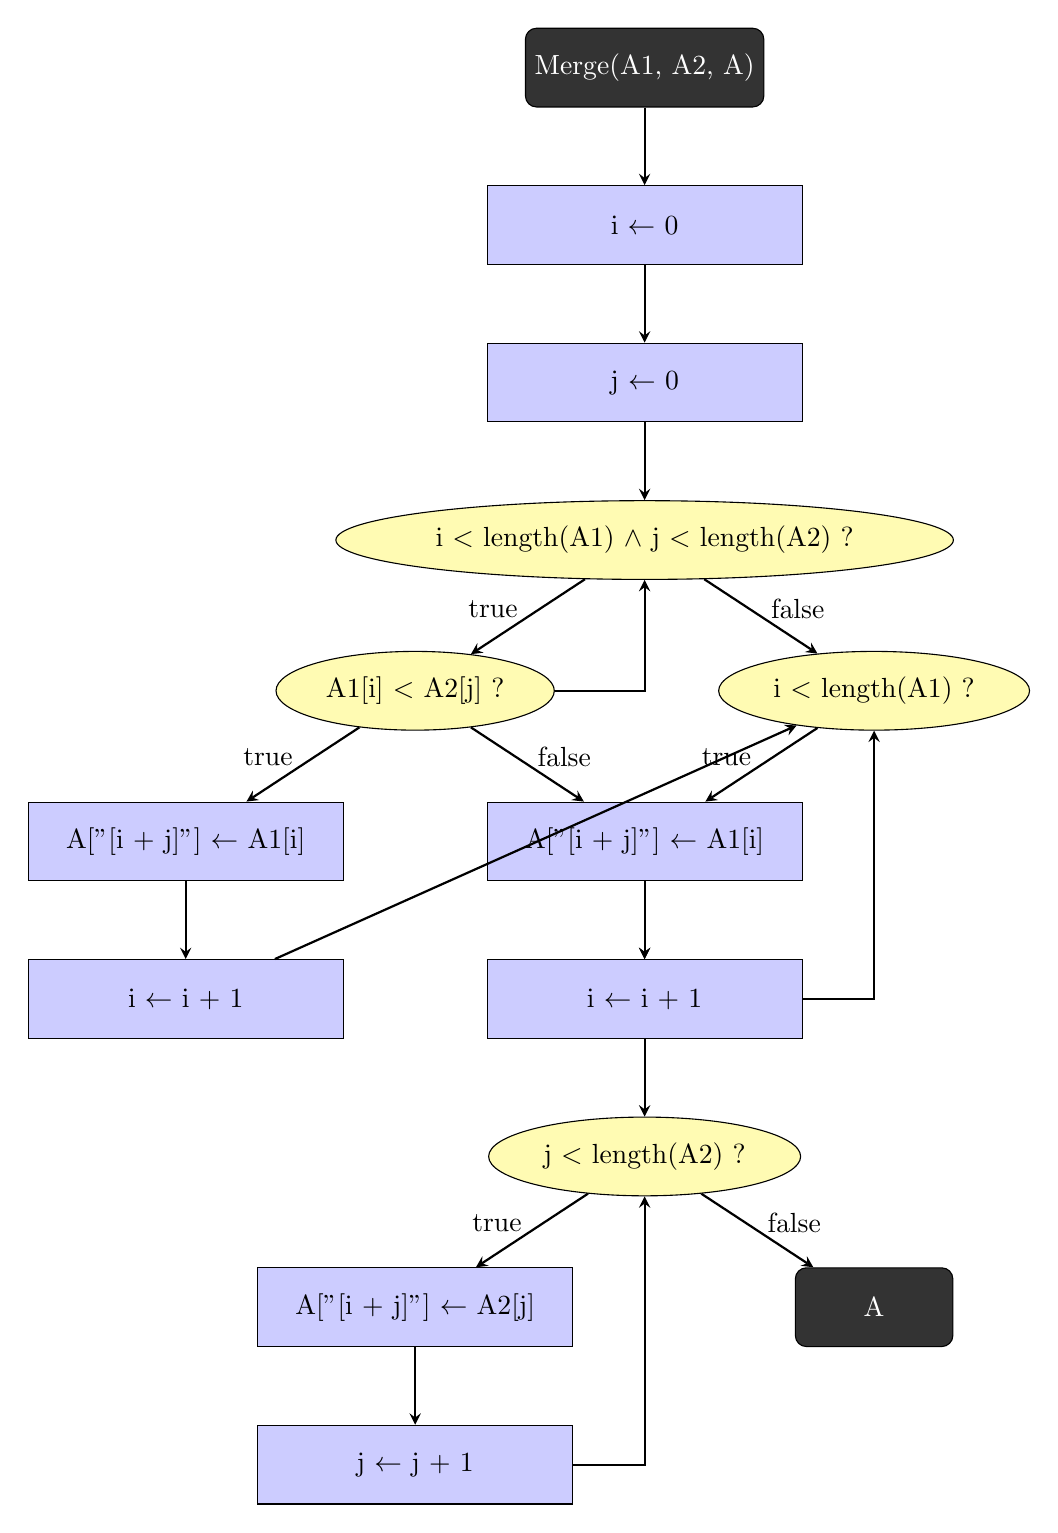
\begin{tikzpicture}[node distance=2cm]

\node (0) [startstop] {Merge(A1, A2, A)};
\node (1) [statement, below of=0] {i $\gets$ 0};
\node (2) [statement, below of=1] {j $\gets$ 0};
\node (3) [decision, below of=2] {i $<$ length(A1) $\land$ j $<$ length(A2) ?};
\node (4) [decision, yshift=-0.5cm, xshift=-1.5cm, below left of=3] {A1[i] $<$ A2[j] ?};
\node (5) [statement, yshift=-0.5cm, xshift=-1.5cm, below left of=4] {A["[i + j]"] $\gets$ A1[i]};
\node (6) [statement, below of=5] {i $\gets$ i + 1};
\node (7) [statement, yshift=-0.5cm, xshift=1.5cm, below right of=4] {A["[i + j]"] $\gets$ A2[j]};
\node (8) [statement, below of=7] {j $\gets$ j + 1};
\node (9) [decision, yshift=-0.5cm, xshift=1.5cm, below right of=3] {i $<$ length(A1) ?};
\node (10) [statement, yshift=-0.5cm, xshift=-1.5cm, below left of=9] {A["[i + j]"] $\gets$ A1[i]};
\node (11) [statement, below of=10] {i $\gets$ i + 1};
\node (12) [decision, below of=11] {j $<$ length(A2) ?};
\node (13) [statement, yshift=-0.5cm, xshift=-1.5cm, below left of=12] {A["[i + j]"] $\gets$ A2[j]};
\node (14) [statement, below of=13] {j $\gets$ j + 1};
\node (15) [startstop, yshift=-0.5cm, xshift=1.5cm, below right of=12] {A};

\draw [edge] (0) -- (1);
\draw [edge] (1) -- (2);
\draw [edge] (2) -- (3);
\draw [edge] (3) -- node[anchor=west, yshift=0.1cm]{false} (9);
\draw [edge] (3) -- node[anchor=east, yshift=0.1cm]{true} (4);
\draw [edge] (4) -| (3);
\draw [edge] (4) -- node[anchor=west, yshift=0.1cm]{false} (7);
\draw [edge] (4) -- node[anchor=east, yshift=0.1cm]{true} (5);
\draw [edge] (5) -- (6);
\draw [edge] (6) -- (9);
\draw [edge] (7) -- (8);
\draw [edge] (9) -- node[anchor=east, yshift=0.1cm]{true} (10);
\draw [edge] (10) -- (11);
\draw [edge] (11) -- (12);
\draw [edge] (11) -| (9);
\draw [edge] (12) -- node[anchor=west, yshift=0.1cm]{false} (15);
\draw [edge] (12) -- node[anchor=east, yshift=0.1cm]{true} (13);
\draw [edge] (13) -- (14);
\draw [edge] (14) -| (12);

\end{tikzpicture}
\end{document}